\chapter{Human affect understanding through multimodal context driven fusion}
In the previous chapter, we explored how visual scene context information can be extracted from multimodal sources, especially media content, by utilizing large-scale pretrained external multimodal models. In this chapter, we will investigate the usage of contextual signals for instance-level multimodal content understanding. We consider instance-level multimodal content understanding along the granularity of individual persons and their perceived affective states in the scene. 
\section{Human affect understanding}
 There has been increased interest in understanding the affective processes associated with various facets of human emotions \cite{dukes2021}. An integral part of affective understanding is the ability to infer expressions of human emotions from various sources like images \cite{AICA}, speech \cite{speechemo}, and language use \cite{Poria2019EmotionRI}, as seen in Fig \ref{}. Affect recognition systems have enabled multiple human-centered applications, notably in healthcare (depression detection \cite{depressiondetection}, autism-spectrum diagnosis \cite{autismguha}) and learning \cite{savchecnkoengagement}).

\begin{figure}[h!]
    \centering
    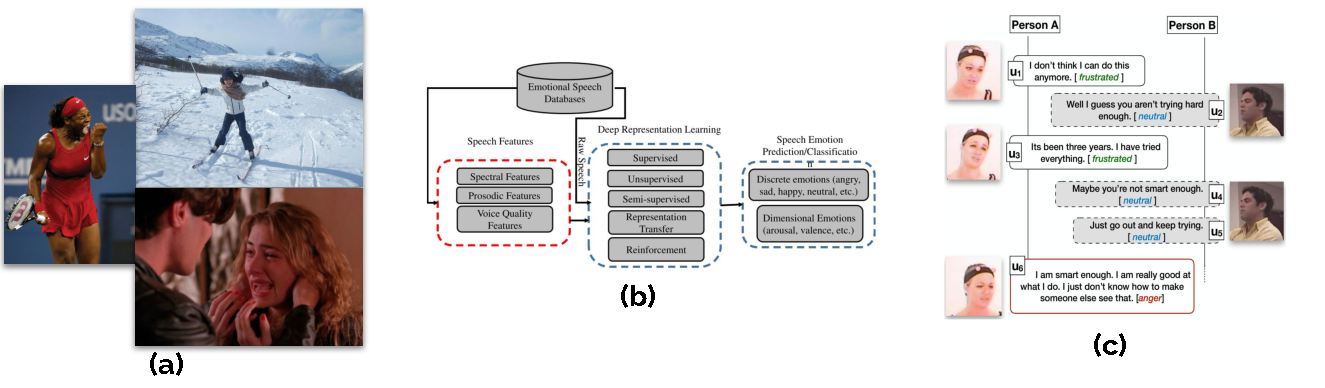
\includegraphics[width=\textwidth]{figures/emotion_overview.pdf}
    \caption{Overview of sources associated with different modalities (mentioned in brackets). \textbf{(a)} images (\textbf{visual}) \textbf{(b)} speech (\textbf{audio}) \textbf{(c)} language (\textbf{language}).}
    \label{emotion overview}
\end{figure}

 
\subsection{Facial expression - Is it the complete picture?}

Affect recognition from images has primarily focused on facial expressions \cite{DFEW,Mollahosseini2019AffectNetAD} along a fixed set of categories. Moreover, facial expression-based methods typically consider crops of a single face, which might provide ambiguous signals for classifying perceived emotions. An example where the face crop doesn't provide a complete picture for decoding the human affective state is shown in Fig \ref{face crop}. In Fig \ref{face crop} (a), we can see that the face crop for the child indicates a perceived affective state of surprise. But after including the entire global scene context, it can be inferred that the child is feeling happy and excited due to the event, i.e., birthday.
Further, in Fig \ref{face crop} (b), we can see that the face crop provides a noisy and incomplete picture. After taking into account the surrounding context that involves a troublesome situation of flooding, it can be assumed that the woman is feeling annoyed. Hence, in this work, we aim to include contextual cues from the visual scene and foreground interactions that contribute to the perception of affective state.

\begin{figure}[h!]
    \centering
    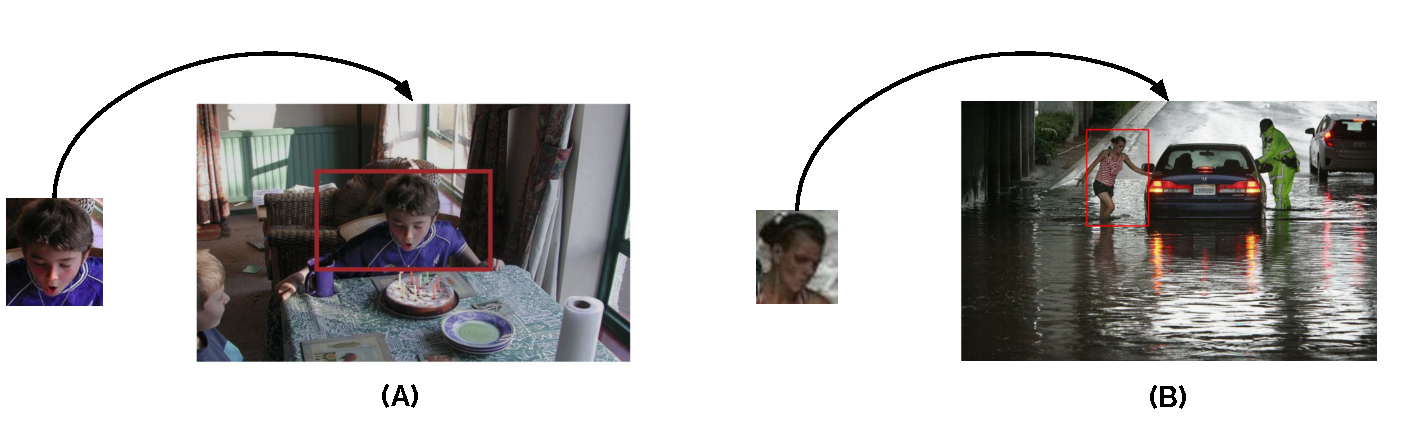
\includegraphics[width=\textwidth]{figures/face_crop_drawings.pdf}
    \caption{Examples from \textbf{EMOTIC} dataset where \textbf{(a)} face crop only provides an incomplete picture \textbf{(b)} face crop provides a noisy signal }
    \label{face crop}
\end{figure}


\section{Role of context in affect perception}
\section{Contextual signals as multi-modal streams:}
\subsection{Visual scene context}
\subsection{Person-specific context}
\subsection{Language-driven foreground context}
\section{Multimodal context fusion module}
\section{Experiments and Results}
\subsection{Emotic}
\subsection{CAER-S}
\subsection{Results}
\subsubsection{Comparisons with state of the art}
\subsubsection{Ablation studies}
\subsubsection{Qualitative examples}
\section{Limitations}
\section{Conclusion}


